```latex
% !TEX root = ../main.tex
\chapter{Examen Julio 2013 - Convocatoria Extraordinaria}
\label{chap:2013_jul_ext}

% ======================================================================
\section{Opción A}
\label{sec:A_2013_jul_ext}
% ======================================================================

\subsection{Bloque I - Cuestión}
\label{subsec:A1_2013_jul_ext}

\begin{cajaenunciado}
La energía cinética de una partícula se incrementa en 1500 J por la acción de una fuerza conservativa. Deduce razonadamente la variación de la energía mecánica y la variación de la energía potencial de la partícula.
\end{cajaenunciado}
\hrule

\subsubsection*{1. Tratamiento de datos y lectura}
\begin{itemize}
    \item \textbf{Tipo de fuerza actuante:} Exclusivamente una fuerza conservativa.
    \item \textbf{Variación de la energía cinética ($\Delta E_c$):} Se produce un incremento, por lo que la variación es positiva. $\Delta E_c = +1500\,\text{J}$.
    \item \textbf{Incógnitas:}
    \begin{itemize}
        \item Variación de la energía mecánica ($\Delta E_M$).
        \item Variación de la energía potencial ($\Delta E_p$).
    \end{itemize}
\end{itemize}

\subsubsection*{2. Representación Gráfica}
\begin{figure}[H]
    \centering
    \fbox{\parbox{0.7\textwidth}{\centering \textbf{Conservación de la Energía Mecánica} \vspace{0.5cm} 
    \vspace{0.5cm} 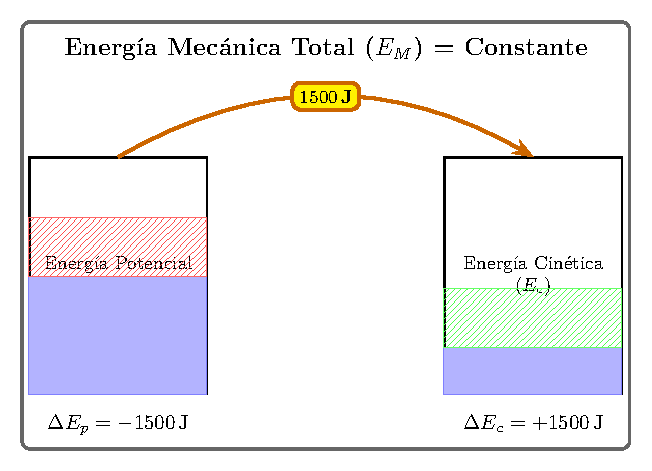
\includegraphics[width=0.9\linewidth]{SelectivosRESUELTOS2025/esquemas/Julio2013/1a.pdf}
    }}
    \caption{Esquema de la transferencia de energía potencial a cinética.}
\end{figure}

\subsubsection*{3. Leyes y Fundamentos Físicos}
El problema se resuelve aplicando el \textbf{Principio de Conservación de la Energía Mecánica}.
\begin{itemize}
    \item Cuando sobre una partícula actúan únicamente fuerzas conservativas (como la gravitatoria o la elástica), su energía mecánica total ($E_M$) permanece constante. La energía mecánica es la suma de la energía cinética ($E_c$) y la energía potencial ($E_p$).
    \item Si la energía mecánica es constante, su variación a lo largo del proceso es nula: $\Delta E_M = 0$.
    \item La variación de la energía mecánica es también la suma de las variaciones de las energías cinética y potencial: $\Delta E_M = \Delta E_c + \Delta E_p$.
\end{itemize}

\subsubsection*{4. Tratamiento Simbólico de las Ecuaciones}
\paragraph{Variación de la Energía Mecánica}
Por la definición de un sistema conservativo:
\begin{gather}
    \Delta E_M = 0
\end{gather}

\paragraph{Variación de la Energía Potencial}
A partir de la constancia de la energía mecánica:
\begin{gather}
    \Delta E_M = \Delta E_c + \Delta E_p = 0
\end{gather}
De esta ecuación, podemos despejar la variación de la energía potencial en función de la variación de la energía cinética:
\begin{gather}
    \Delta E_p = -\Delta E_c
\end{gather}

\subsubsection*{5. Sustitución Numérica y Resultado}
\begin{cajaresultado}
Al actuar solo una fuerza conservativa, la energía mecánica se conserva. Por tanto, su variación es \textbf{nula}: $\boldsymbol{\Delta E_M = 0\,\textbf{J}}$.
\end{cajaresultado}

\paragraph{Variación de la Energía Potencial}
Sustituimos el dato del problema en la ecuación simbólica:
\begin{gather}
    \Delta E_p = -(+1500\,\text{J}) = -1500\,\text{J}
\end{gather}
\begin{cajaresultado}
La variación de la energía potencial es $\boldsymbol{\Delta E_p = -1500\,\textbf{J}}$.
\end{cajaresultado}

\subsubsection*{6. Conclusión}
\begin{cajaconclusion}
En un sistema conservativo, la energía no se crea ni se destruye, solo se transforma entre sus formas cinética y potencial. El incremento de 1500 J en la energía cinética se ha producido a costa de una disminución de 1500 J en la energía potencial, manteniendo la energía mecánica total constante.
\end{cajaconclusion}

\newpage

\subsection{Bloque II - Problema}
\label{subsec:A2_2013_jul_ext}

\begin{cajaenunciado}
Una onda transversal se propaga por una cuerda según la ecuación $y(x,t)=0,4\cos[10\pi(2t-x)]$, en unidades del SI. Calcula:
\begin{enumerate}
    \item[a)] La elongación, y, del punto de la cuerda situado en $x=20$ cm en el instante $t=0,5$ s. (1 punto)
    \item[b)] La velocidad transversal de dicho punto en ese mismo instante $t=0,5$ s. (1 punto)
\end{enumerate}
\end{cajaenunciado}
\hrule

\subsubsection*{1. Tratamiento de datos y lectura}
La ecuación de la onda se proporciona en unidades del Sistema Internacional. Es conveniente expandirla para identificar sus parámetros.
\begin{itemize}
    \item \textbf{Ecuación de la onda:} $y(x,t) = 0,4\cos[20\pi t - 10\pi x]$.
    \item Al compararla con la forma general $y(x,t) = A\cos(\omega t - kx)$, identificamos:
        \begin{itemize}
            \item \textbf{Amplitud ($A$):} $A = 0,4\,\text{m}$.
            \item \textbf{Frecuencia angular ($\omega$):} $\omega = 20\pi\,\text{rad/s}$.
            \item \textbf{Número de onda ($k$):} $k = 10\pi\,\text{rad/m}$.
        \end{itemize}
    \item \textbf{Posición para el cálculo ($x$):} $x = 20\,\text{cm} = 0,2\,\text{m}$.
    \item \textbf{Instante para el cálculo ($t$):} $t = 0,5\,\text{s}$.
    \item \textbf{Incógnitas:} Elongación $y(0.2, 0.5)$ y velocidad transversal $v_y(0.2, 0.5)$.
\end{itemize}

\subsubsection*{2. Representación Gráfica}
\begin{figure}[H]
    \centering
    \fbox{\parbox{1.2\textwidth}{\centering \textbf{Onda Transversal} \vspace{0.5cm} 
    \vspace{0.5cm} 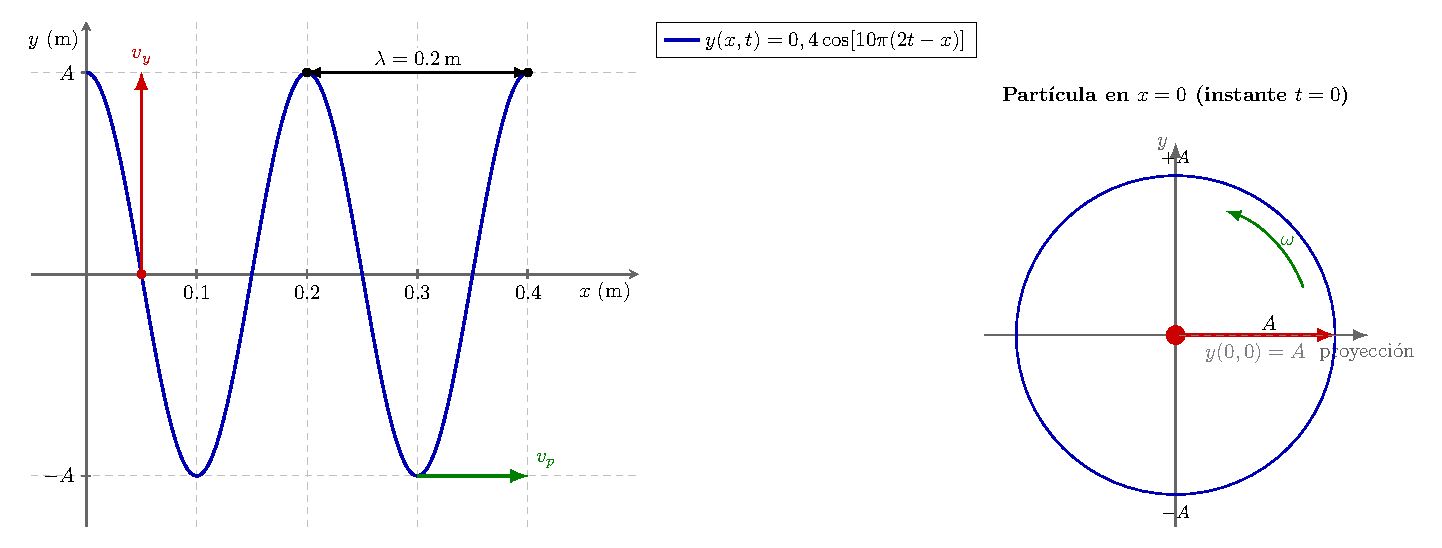
\includegraphics[width=1.2\linewidth]{SelectivosRESUELTOS2025/esquemas/Julio2013/2a.pdf}
    }}
    \caption{Representación de una onda armónica y la velocidad transversal de un punto.}
\end{figure}

\subsubsection*{3. Leyes y Fundamentos Físicos}
\paragraph{a) Elongación}
La elongación $y$ de un punto de la cuerda en una posición $x$ y un instante $t$ se calcula directamente sustituyendo estos valores en la ecuación de la onda proporcionada.

\paragraph{b) Velocidad transversal}
La velocidad transversal ($v_y$) de un punto de la cuerda no es la velocidad de propagación de la onda, sino la velocidad con la que ese punto oscila verticalmente. Se obtiene derivando la función de elongación $y(x,t)$ con respecto al tiempo $t$.
$$ v_y(x,t) = \frac{\partial y(x,t)}{\partial t} $$

\subsubsection*{4. Tratamiento Simbólico de las Ecuaciones}
\paragraph{a) Elongación}
La ecuación ya está dada:
\begin{gather}
    y(x,t) = 0,4\cos(20\pi t - 10\pi x)
\end{gather}

\paragraph{b) Velocidad transversal}
Derivamos la expresión anterior respecto al tiempo:
\begin{gather}
    v_y(x,t) = \frac{\partial}{\partial t} [0,4\cos(20\pi t - 10\pi x)] = 0,4 \cdot (-\sin(20\pi t - 10\pi x)) \cdot (20\pi) \nonumber \\
    v_y(x,t) = -8\pi \sin(20\pi t - 10\pi x)
\end{gather}

\subsubsection*{5. Sustitución Numérica y Resultado}
\paragraph{a) Elongación en $x=0,2$ m y $t=0,5$ s}
Sustituimos los valores en la ecuación de la elongación:
\begin{gather}
    y(0.2, 0.5) = 0,4\cos(20\pi \cdot 0,5 - 10\pi \cdot 0,2) = 0,4\cos(10\pi - 2\pi) \nonumber \\
    y(0.2, 0.5) = 0,4\cos(8\pi)
\end{gather}
Dado que el coseno de cualquier múltiplo entero de $2\pi$ es 1, $\cos(8\pi)=1$.
\begin{gather}
    y(0.2, 0.5) = 0,4 \cdot 1 = 0,4\,\text{m}
\end{gather}
\begin{cajaresultado}
La elongación del punto es $\boldsymbol{y = 0,4\,\textbf{m}}$.
\end{cajaresultado}

\paragraph{b) Velocidad transversal en $x=0,2$ m y $t=0,5$ s}
Sustituimos los valores en la ecuación de la velocidad:
\begin{gather}
    v_y(0.2, 0.5) = -8\pi \sin(20\pi \cdot 0,5 - 10\pi \cdot 0,2) = -8\pi \sin(8\pi)
\end{gather}
Dado que el seno de cualquier múltiplo entero de $\pi$ es 0, $\sin(8\pi)=0$.
\begin{gather}
    v_y(0.2, 0.5) = -8\pi \cdot 0 = 0\,\text{m/s}
\end{gather}
\begin{cajaresultado}
La velocidad transversal del punto en ese instante es $\boldsymbol{v_y = 0\,\textbf{m/s}}$.
\end{cajaresultado}

\subsubsection*{6. Conclusión}
\begin{cajaconclusion}
En el instante $t=0,5$ s, el punto de la cuerda situado en $x=0,2$ m se encuentra en su máxima elongación positiva, es decir, en una cresta de la onda ($y=A=0,4$ m). Como en todos los movimientos armónicos, en el punto de máxima elongación la velocidad instantánea es nula, ya que la partícula se detiene para invertir el sentido de su movimiento.
\end{cajaconclusion}

\newpage

\subsection{Bloque III - Cuestión}
\label{subsec:A3_2013_jul_ext}

\begin{cajaenunciado}
En el esquema adjunto se representa un objeto de altura y, así como su imagen, de altura y', proporcionada por una lente delgada convergente. Determina, explicando el procedimiento seguido, la distancia focal imagen f' de la lente ¿La imagen es real o virtual? ¿Cuál es el aumento lateral que proporciona la lente para ese objeto?
\textbf{Nota:} cada una de las divisiones (horizontales y verticales) equivale a 10 cm.
\end{cajaenunciado}
\hrule

\subsubsection*{1. Tratamiento de datos y lectura}
Se extraen los datos directamente de la imagen, usando la escala proporcionada (1 división = 10 cm) y el convenio de signos DIN (lente en el origen, luz de izquierda a derecha).
\begin{itemize}
    \item \textbf{Posición del objeto ($s$):} El objeto está 2 divisiones a la izquierda de la lente. $s = -2 \times 10\,\text{cm} = -20\,\text{cm}$.
    \item \textbf{Altura del objeto ($y$):} El objeto tiene una altura de 2 divisiones. $y = +2 \times 10\,\text{cm} = +20\,\text{cm}$.
    \item \textbf{Posición de la imagen ($s'$):} La imagen está 2 divisiones a la izquierda de la lente. $s' = -2 \times 10\,\text{cm} = -20\,\text{cm}$.
    \item \textbf{Altura de la imagen ($y'$):} La imagen tiene una altura de 4 divisiones. $y' = +4 \times 10\,\text{cm} = +40\,\text{cm}$.
    \item \textbf{Incógnitas:} Distancia focal imagen ($f'$), naturaleza de la imagen (real o virtual), y aumento lateral ($M_L$).
\end{itemize}

\subsubsection*{2. Representación Gráfica}
\begin{figure}[H]
    \centering
    \fbox{\parbox{0.8\textwidth}{\centering \textbf{Trazado de rayos para lente convergente (lupa)} \vspace{0.5cm} 
    \vspace{0.5cm} 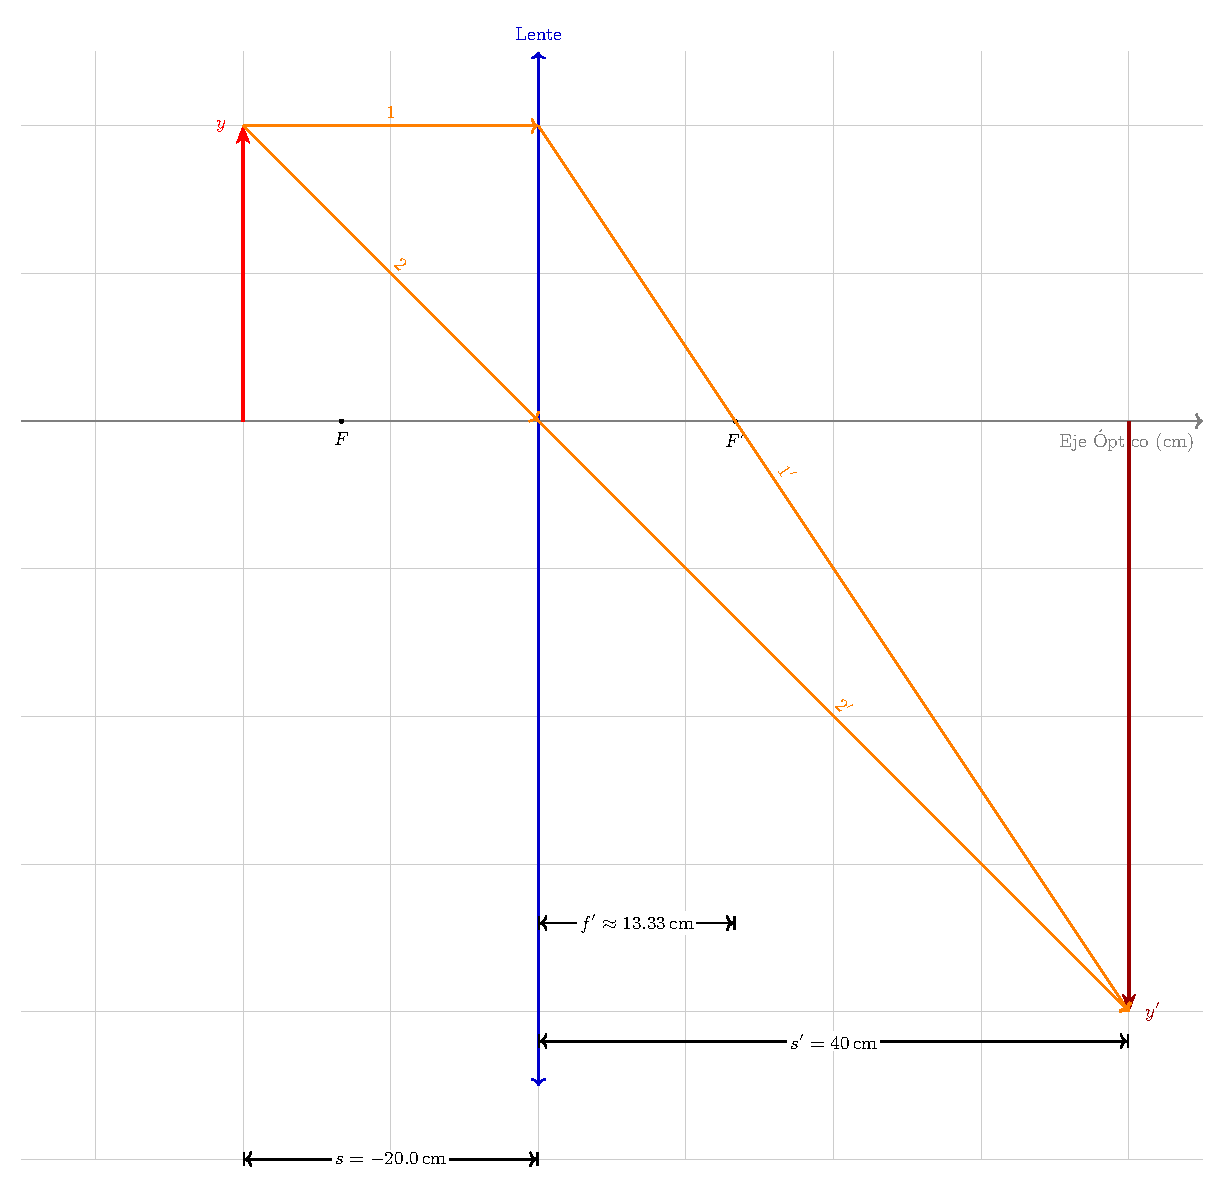
\includegraphics[width=0.9\linewidth]{SelectivosRESUELTOS2025/esquemas/Julio2013/3a.pdf}
    }}
    \caption{Análisis gráfico del sistema lente-objeto-imagen.}
\end{figure}

\subsubsection*{3. Leyes y Fundamentos Físicos}
Para resolver el problema se utilizan las ecuaciones fundamentales de las lentes delgadas:
\begin{itemize}
    \item \textbf{Ecuación de Gauss para lentes delgadas:} Relaciona las posiciones del objeto ($s$) y la imagen ($s'$) con la distancia focal imagen ($f'$).
    $$ \frac{1}{s'} - \frac{1}{s} = \frac{1}{f'} $$
    \item \textbf{Ecuación del Aumento Lateral ($M_L$):} Relaciona los tamaños y posiciones de la imagen y el objeto.
    $$ M_L = \frac{y'}{y} = \frac{s'}{s} $$
    \item \textbf{Naturaleza de la imagen:} La imagen es \textbf{virtual} si se forma en el mismo lado de la lente que el objeto (a la izquierda, $s'<0$). Es \textbf{real} si se forma en el lado opuesto ($s'>0$).
\end{itemize}

\subsubsection*{4. Tratamiento Simbólico de las Ecuaciones}
\paragraph{Distancia Focal Imagen ($f'$)}
Se despeja $f'$ de la ecuación de Gauss:
\begin{gather}
    f' = \left(\frac{1}{s'} - \frac{1}{s}\right)^{-1} = \frac{s \cdot s'}{s - s'}
\end{gather}

\paragraph{Naturaleza de la imagen}
Se determina observando el signo de $s'$.

\paragraph{Aumento Lateral ($M_L$)}
Se calcula a partir de las alturas o de las posiciones:
\begin{gather}
    M_L = \frac{y'}{y}
\end{gather}

\subsubsection*{5. Sustitución Numérica y Resultado}
\paragraph{Distancia Focal Imagen ($f'$)}


Datos:
\begin{itemize}
    \item \textbf{Posición del objeto ($s$):} $s = -2 \times 10\,\text{cm} = -20\,\text{cm}$.
    \item \textbf{Altura del objeto ($y$):} $y = +2 \times 10\,\text{cm} = +20\,\text{cm}$.
    \item \textbf{Posición de la imagen ($s'$):} $s' = +4 \times 10\,\text{cm} = +40\,\text{cm}$.
    \item \textbf{Altura de la imagen ($y'$):} $y' = -4 \times 10\,\text{cm} = -40\,\text{cm}$.
\end{itemize}

\paragraph{Distancia Focal Imagen ($f'$)}
\begin{gather}
    \frac{1}{f'} = \frac{1}{s'} - \frac{1}{s} = \frac{1}{+40} - \frac{1}{-20} = \frac{1}{40} + \frac{2}{40} = \frac{3}{40} \nonumber \\
    f' = \frac{40}{3} \approx +13,33\,\text{cm}
\end{gather}
\begin{cajaresultado}
La distancia focal imagen de la lente es $\boldsymbol{f' \approx +13,33\,\textbf{cm}}$.
\end{cajaresultado}

\paragraph{Naturaleza de la imagen}
Como la posición de la imagen $s' = +40\,\text{cm}$ es positiva, la imagen se forma a la derecha de la lente.
\begin{cajaresultado}
La imagen es \textbf{Real}.
\end{cajaresultado}

\paragraph{Aumento Lateral ($M_L$)}
\begin{gather}
    M_L = \frac{y'}{y} = \frac{-40\,\text{cm}}{+20\,\text{cm}} = -2
\end{gather}
(Comprobación: $M_L = s'/s = +40/(-20) = -2$). El resultado es consistente.
\begin{cajaresultado}
El aumento lateral es $\boldsymbol{M_L = -2}$.
\end{cajaresultado}


\subsubsection*{6. Conclusión}
\begin{cajaconclusion}
Interpretando las posiciones y tamaños del objeto y la imagen a partir de la cuadrícula, se han aplicado las ecuaciones de las lentes delgadas. Se deduce que se trata de una lente convergente con una distancia focal de +13,33 cm. La imagen formada es real (ya que $s'>0$), invertida (como se ve en la figura y confirma $M_L<0$) y de doble tamaño que el objeto ($M_L=-2$).
\end{cajaconclusion}

\newpage

\subsection{Bloque IV - Problema}
\label{subsec:A4_2013_jul_ext}

\begin{cajaenunciado}
Dos cargas eléctricas $q_1 = 5\,\mu\text{C}$ y $q_2 = -3\,\mu\text{C}$ se encuentran en las posiciones (0,0) m y (4,0) m respectivamente, como muestra la figura. Calcula:
\begin{enumerate}
    \item[a)] El vector campo eléctrico en el punto B (4,-3) m. (1 punto)
    \item[b)] El potencial eléctrico en el punto A (2,0) m. Determina también el trabajo para trasladar una carga de $-10^{-12}\,\text{C}$ desde el infinito hasta el punto A. (Considera nulo el potencial eléctrico en el infinito). (1 punto)
\end{enumerate}
\textbf{Dato:} constante de Coulomb, $k = 9 \cdot 10^9 \, \text{N}\text{m}^2/\text{C}^2$.
\end{cajaenunciado}
\hrule

\subsubsection*{1. Tratamiento de datos y lectura}
\begin{itemize}
    \item \textbf{Carga 1 ($q_1$):} $q_1 = +5\,\mu\text{C} = 5 \cdot 10^{-6}\,\text{C}$, en $P_1(0,0)$.
    \item \textbf{Carga 2 ($q_2$):} $q_2 = -3\,\mu\text{C} = -3 \cdot 10^{-6}\,\text{C}$, en $P_2(4,0)$.
    \item \textbf{Punto para campo ($B$):} $B(4,-3)$.
    \item \textbf{Punto para potencial ($A$):} $A(2,0)$.
    \item \textbf{Carga de prueba ($q'$):} $q' = -10^{-12}\,\text{C}$.
    \item \textbf{Constante de Coulomb ($k$):} $k = 9 \cdot 10^9 \, \text{N}\text{m}^2/\text{C}^2$.
    \item \textbf{Incógnitas:} $\vec{E}_B$, $V_A$, $W_{\infty \to A}$.
\end{itemize}

\subsubsection*{2. Representación Gráfica}
\begin{figure}[H]
    \centering
    \fbox{\parbox{0.8\textwidth}{\centering 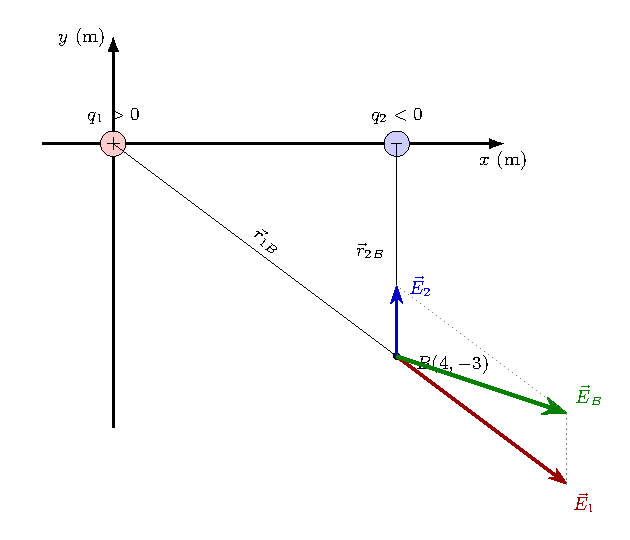
\includegraphics[width=0.9\linewidth]{SelectivosRESUELTOS2025/esquemas/Julio2013/4a.pdf}
    }}
    \caption{Superposición de los campos eléctricos creados por $q_1$ y $q_2$ en el punto B.}
\end{figure}
\begin{figure}[H]
    \centering
    \fbox{\parbox{0.8\textwidth}{\centering \textbf{b) Potencial eléctrico en A} \vspace{0.5cm} 
    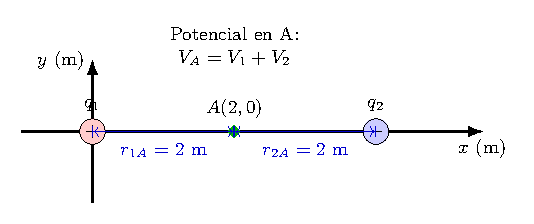
\includegraphics[width=0.9\linewidth]{SelectivosRESUELTOS2025/esquemas/Julio2013/4a(b).pdf}
    }}
    \caption{Puntos y distancias para el cálculo del potencial eléctrico en A.}
\end{figure}

\subsubsection*{3. Leyes y Fundamentos Físicos}
\paragraph{a) Campo Eléctrico}
Se aplica el \textbf{Principio de Superposición}. El campo eléctrico total en el punto B es la suma vectorial de los campos creados por cada carga individualmente: $\vec{E}_B = \vec{E}_{1,B} + \vec{E}_{2,B}$. El campo creado por una carga puntual $q$ es $\vec{E} = k\frac{q}{r^2}\vec{u}_r$.

\paragraph{b) Potencial Eléctrico y Trabajo}
El potencial eléctrico en A es la suma escalar de los potenciales creados por cada carga: $V_A = V_{1,A} + V_{2,A}$. El potencial creado por una carga puntual es $V = k\frac{q}{r}$. El trabajo realizado por un agente externo para mover una carga $q'$ desde el infinito hasta el punto A es $W_{\infty \to A} = q'\Delta V = q'(V_A - V_\infty)$. Por convenio, $V_\infty=0$, por lo que $W_{\infty \to A} = q'V_A$.

\subsubsection*{4. Tratamiento Simbólico de las Ecuaciones}
\paragraph{a) Campo eléctrico en B(4,-3)}
\begin{itemize}
    \item Distancia de $q_1$ a B: $\vec{r}_{1B} = (4-0)\vec{i} + (-3-0)\vec{j} = 4\vec{i}-3\vec{j}$. Módulo: $r_{1B} = \sqrt{4^2+(-3)^2}=5\,\text{m}$. Vector unitario: $\vec{u}_{1B} = \frac{4\vec{i}-3\vec{j}}{5}$.
    \item Distancia de $q_2$ a B: $\vec{r}_{2B} = (4-4)\vec{i} + (-3-0)\vec{j} = -3\vec{j}$. Módulo: $r_{2B}=3\,\text{m}$. Vector unitario: $\vec{u}_{2B} = -\vec{j}$.
\end{itemize}
$\vec{E}_B = k\frac{q_1}{r_{1B}^2}\vec{u}_{1B} + k\frac{q_2}{r_{2B}^2}\vec{u}_{2B}$.

\paragraph{b) Potencial en A(2,0) y Trabajo}
\begin{itemize}
    \item Distancia de $q_1$ a A: $r_{1A} = 2\,\text{m}$.
    \item Distancia de $q_2$ a A: $r_{2A} = 4-2 = 2\,\text{m}$.
\end{itemize}
$V_A = k\frac{q_1}{r_{1A}} + k\frac{q_2}{r_{2A}}$.
$W_{\infty \to A} = q'V_A$.

\subsubsection*{5. Sustitución Numérica y Resultado}
\paragraph{a) Campo eléctrico en B(4,-3)}
\begin{gather}
    \vec{E}_{1,B} = (9\cdot10^9)\frac{5\cdot10^{-6}}{5^2}\frac{4\vec{i}-3\vec{j}}{5} = 1800 \cdot (0,8\vec{i}-0,6\vec{j}) = 1440\vec{i} - 1080\vec{j}\,\text{N/C} \\
   \\ \vec{E}_{2,B} = (9\cdot10^9)\frac{-3\cdot10^{-6}}{3^2}(-\vec{j}) = (-3000)(-\vec{j}) = 3000\vec{j}\,\text{N/C} \\
   \\ \vec{E}_B = (1440\vec{i} - 1080\vec{j}) + 3000\vec{j} = 1440\vec{i} + 1920\vec{j}\,\text{N/C}
\end{gather}
\begin{cajaresultado}
El vector campo eléctrico en el punto B es $\boldsymbol{\vec{E}_B = (1440\vec{i} + 1920\vec{j})\,\textbf{N/C}}$.
\end{cajaresultado}

\paragraph{b) Potencial en A(2,0) y Trabajo}
\begin{gather}
    V_A = (9\cdot10^9)\frac{5\cdot10^{-6}}{2} + (9\cdot10^9)\frac{-3\cdot10^{-6}}{2} = 22500 - 13500 = 9000\,\text{V} \\
\\    W_{\infty \to A} = q'V_A = (-10^{-12}\,\text{C}) \cdot (9000\,\text{V}) = -9 \cdot 10^{-9}\,\text{J}
\end{gather}
\begin{cajaresultado}
El potencial eléctrico en A es $\boldsymbol{V_A = 9000\,\textbf{V}}$ y el trabajo para trasladar la carga es $\boldsymbol{W = -9 \cdot 10^{-9}\,\textbf{J}}$.
\end{cajaresultado}

\subsubsection*{6. Conclusión}
\begin{cajaconclusion}
Aplicando el principio de superposición, se ha calculado el campo eléctrico vectorial en el punto B y el potencial escalar en el punto A. El trabajo necesario para traer la carga de prueba desde el infinito es negativo, lo que indica que el campo eléctrico realiza un trabajo positivo; la carga negativa es atraída hacia la región de potencial positivo.
\end{cajaconclusion}

\newpage

\subsection{Bloque V - Cuestión}
\label{subsec:A5_2013_jul_ext}

\begin{cajaenunciado}
En el sincrotrón ALBA (sito en Barcelona) se aceleran los electrones hasta una velocidad para la que su masa es 6000 veces el valor de la masa en reposo. Calcula la energía (en julios y en MeV) de los electrones.
\textbf{Datos:} velocidad de la luz en el vacío, $c=3 \cdot 10^8\,\text{m/s}$; masa del electrón, $m_e = 9,1 \cdot 10^{-31}\,\text{kg}$; carga elemental, $e = 1,6 \cdot 10^{-19}\,\text{C}$.
\end{cajaenunciado}
\hrule

\subsubsection*{1. Tratamiento de datos y lectura}
\begin{itemize}
    \item \textbf{Masa relativista del electrón ($m$):} $m = 6000 \cdot m_0$, donde $m_0$ es la masa en reposo.
    \item \textbf{Masa en reposo del electrón ($m_0$):} $m_0 = 9,1 \cdot 10^{-31}\,\text{kg}$.
    \item \textbf{Velocidad de la luz ($c$):} $c = 3 \cdot 10^8\,\text{m/s}$.
    \item \textbf{Carga elemental ($e$):} $e = 1,6 \cdot 10^{-19}\,\text{C}$.
    \item \textbf{Incógnita:} Energía total del electrón ($E$) en Julios y en Mega-electronvoltios (MeV).
\end{itemize}

\subsubsection*{2. Representación Gráfica}
\begin{figure}[H]
    \centering
    \fbox{\parbox{0.7\textwidth}{\centering 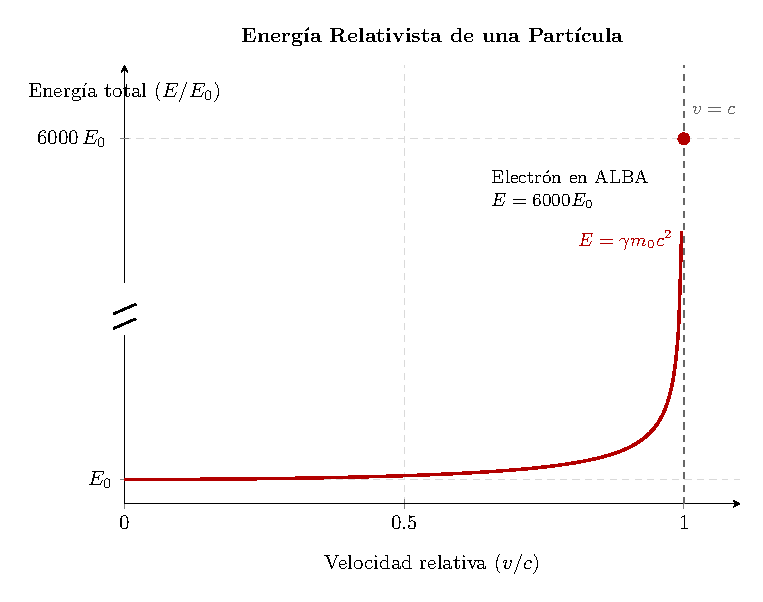
\includegraphics[width=0.9\linewidth]{SelectivosRESUELTOS2025/esquemas/Julio2013/5a.pdf}
    }}
    \caption{Relación entre la energía total y la velocidad de una partícula.}
\end{figure}

\subsubsection*{3. Leyes y Fundamentos Físicos}
El problema se resuelve aplicando la \textbf{Teoría de la Relatividad Especial} de Einstein, concretamente la famosa ecuación de equivalencia masa-energía. La energía total ($E$) de una partícula se relaciona con su masa relativista ($m$) y la velocidad de la luz ($c$) mediante la fórmula:
$$ E = m c^2 $$
La masa relativista ($m$) depende de la velocidad de la partícula y de su masa en reposo ($m_0$) a través del factor de Lorentz, $\gamma$: $m = \gamma m_0$. Por tanto, la energía total también se puede escribir como $E = \gamma m_0 c^2$.

\subsubsection*{4. Tratamiento Simbólico de las Ecuaciones}
La energía total del electrón es:
\begin{gather}
    E = m c^2
\end{gather}
Sustituyendo la relación de masas dada en el enunciado:
\begin{gather}
    E = (6000 \cdot m_0) c^2
\end{gather}
Para convertir la energía de Julios a electronvoltios (eV), se divide por el valor de la carga elemental ($e$). Para convertir a MeV, se divide además por $10^6$.
\begin{gather}
    E\,(\text{MeV}) = \frac{E\,(\text{J})}{e \cdot 10^6}
\end{gather}

\subsubsection*{5. Sustitución Numérica y Resultado}
\paragraph{Energía en Julios}
\begin{gather}
    E = 6000 \cdot (9,1 \cdot 10^{-31}\,\text{kg}) \cdot (3 \cdot 10^8\,\text{m/s})^2 \nonumber \\
    E = 6000 \cdot (9,1 \cdot 10^{-31}) \cdot (9 \cdot 10^{16}) = 4,914 \cdot 10^{-10}\,\text{J}
\end{gather}
\begin{cajaresultado}
La energía de los electrones es $\boldsymbol{E \approx 4,91 \cdot 10^{-10}\,\textbf{J}}$.
\end{cajaresultado}

\paragraph{Energía en MeV}
\begin{gather}
    E\,(\text{MeV}) = \frac{4,914 \cdot 10^{-10}\,\text{J}}{1,6 \cdot 10^{-19}\,\text{C} \cdot 10^6} = \frac{4,914 \cdot 10^{-10}}{1,6 \cdot 10^{-13}} \approx 3071\,\text{MeV}
\end{gather}
\begin{cajaresultado}
La energía de los electrones es $\boldsymbol{E \approx 3071\,\textbf{MeV}}$.
\end{cajaresultado}

\subsubsection*{6. Conclusión}
\begin{cajaconclusion}
El enorme aumento de la masa del electrón (6000 veces su masa en reposo) es una manifestación de su energía extremadamente alta, de acuerdo con la equivalencia masa-energía de Einstein. La energía total de estos electrones ultrarrelativistas es de aproximadamente $4,91 \cdot 10^{-10}$ J, lo que equivale a más de 3000 MeV.
\end{cajaconclusion}

\newpage

\subsection{Bloque VI - Cuestión}
\label{subsec:A6_2013_jul_ext}

\begin{cajaenunciado}
Explica brevemente en qué consisten la radiación alfa y la radiación beta. Halla el número atómico y el número másico del elemento producido a partir del ${}_{82}^{210}\text{Pb}$, después de emitir una partícula $\alpha$ y dos partículas $\beta^{-}$.
\end{cajaenunciado}
\hrule

\subsubsection*{1. Tratamiento de datos y lectura}
\begin{itemize}
    \item \textbf{Tarea 1:} Definir la radiación alfa ($\alpha$) y beta ($\beta$).
    \item \textbf{Núcleo inicial:} Plomo-210, ${}_{82}^{210}\text{Pb}$.
    \item \textbf{Partículas emitidas:} Una partícula $\alpha$ y dos partículas $\beta^{-}$.
    \item \textbf{Incógnita:} Número atómico ($Z'$) y número másico ($A'$) del núcleo final.
\end{itemize}

\subsubsection*{2. Representación Gráfica}
\begin{figure}[H]
    \centering
    \fbox{\parbox{0.8\textwidth}{\centering 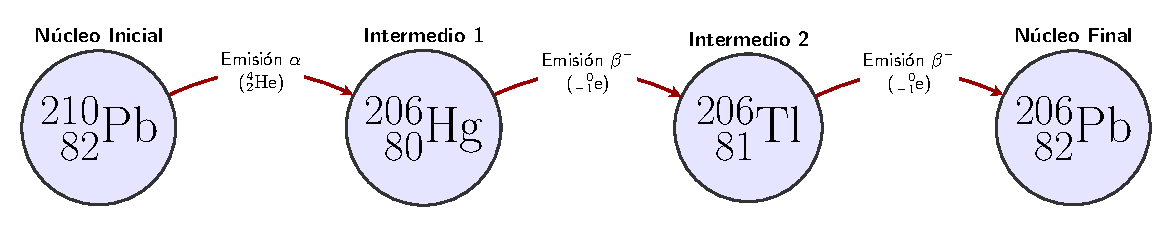
\includegraphics[width=0.9\linewidth]{SelectivosRESUELTOS2025/esquemas/Julio2013/6a.pdf}
    }}
    \caption{Esquema de la desintegración del Plomo-210.}
\end{figure}

\subsubsection*{3. Leyes y Fundamentos Físicos}
\paragraph{Definiciones de las Radiaciones}
\begin{itemize}
    \item \textbf{Radiación alfa ($\alpha$):} Es la emisión de un núcleo de Helio-4 (${}_{2}^{4}\text{He}$), que consta de dos protones y dos neutrones. Es una partícula relativamente pesada y con carga positiva (+2e).
    \item \textbf{Radiación beta menos ($\beta^{-}$):} Es la emisión de un electrón (${}_{-1}^{0}e$) desde el núcleo. Este proceso ocurre cuando un neutrón del núcleo se transforma en un protón, un electrón y un antineutrino. El electrón es expulsado a alta velocidad.
\end{itemize}

\paragraph{Leyes de Conservación de Soddy-Fajans}
En cualquier reacción nuclear, el número másico total (A, suma de protones y neutrones) y el número atómico total (Z, número de protones) deben conservarse.

\subsubsection*{4. Tratamiento Simbólico de las Ecuaciones}
Podemos representar la desintegración completa con una única ecuación nuclear. Sea ${}_{Z'}^{A'}X$ el núcleo final.
\begin{gather}
    {}_{82}^{210}\text{Pb} \longrightarrow {}_{Z'}^{A'}X + {}_{2}^{4}\text{He} + 2 \cdot {}_{-1}^{0}e
\end{gather}
(Nota: Se omite el antineutrino en la notación simplificada).
Ahora aplicamos las leyes de conservación:
\begin{itemize}
    \item \textbf{Conservación del número másico (A):} La suma de los superíndices a ambos lados debe ser igual.
    $$ 210 = A' + 4 + 2 \cdot 0 $$
    \item \textbf{Conservación del número atómico (Z):} La suma de los subíndices a ambos lados debe ser igual.
    $$ 82 = Z' + 2 + 2 \cdot (-1) $$
\end{itemize}

\subsubsection*{5. Sustitución Numérica y Resultado}
\paragraph{Cálculo del número másico final ($A'$)}
\begin{gather}
    210 = A' + 4 \implies A' = 210 - 4 = 206
\end{gather}

\paragraph{Cálculo del número atómico final ($Z'$)}
\begin{gather}
    82 = Z' + 2 - 2 = Z' \implies Z' = 82
\end{gather}
\begin{cajaresultado}
El número másico del elemento producido es $\boldsymbol{A' = 206}$. El número atómico es $\boldsymbol{Z' = 82}$.
\end{cajaresultado}

\subsubsection*{6. Conclusión}
\begin{cajaconclusion}
La emisión de una partícula alfa reduce el número másico en 4 unidades y el número atómico en 2. La emisión de dos partículas beta no altera el número másico, pero aumenta el número atómico en 2 unidades (ya que dos neutrones se convierten en protones). El efecto neto es una disminución de 4 en el número másico y de 0 en el número atómico. El núcleo final es, por tanto, ${}_{82}^{206}\text{Pb}$, otro isótopo del plomo.
\end{cajaconclusion}

\newpage

% ======================================================================
\section{Opción B}
\label{sec:B_2013_jul_ext}
% ======================================================================

\subsection{Bloque I - Problema}
\label{subsec:B1_2013_jul_ext}

\begin{cajaenunciado}
Tres planetas se encuentran situados, en un cierto instante, en las posiciones representadas en la figura, siendo $a = 10^5$ m. Considerando que son masas puntuales de valores $m_2=m_3=2m_1=2 \cdot 10^{21}$ kg, calcula:
\begin{enumerate}
    \item[a)] El vector campo gravitatorio originado por los 3 planetas en el punto O(0,0) m. (1 punto)
    \item[b)] El potencial gravitatorio (energía potencial por unidad de masa) originado por los 3 planetas en el punto P(a,0) m. (1 punto)
\end{enumerate}
\textbf{Dato:} constante de gravitación universal, $G = 6,67 \cdot 10^{-11} \, \text{N}\text{m}^2/\text{kg}^2$.
\end{cajaenunciado}
\hrule

\subsubsection*{1. Tratamiento de datos y lectura}
\begin{itemize}
    \item \textbf{Masas y posiciones:}
        \begin{itemize}
            \item $m_1$: en $P_1(-a, 0)$. Su masa es $m_1 = (2 \cdot 10^{21})/2 = 1 \cdot 10^{21}\,\text{kg}$.
            \item $m_2$: en $P_2(0, -a)$. Su masa es $m_2 = 2 \cdot 10^{21}\,\text{kg}$.
            \item $m_3$: en $P_3(0, a)$. Su masa es $m_3 = 2 \cdot 10^{21}\,\text{kg}$.
        \end{itemize}
    \item \textbf{Distancia característica ($a$):} $a = 10^5\,\text{m}$.
    \item \textbf{Punto para campo:} Origen O(0,0).
    \item \textbf{Punto para potencial:} P(a,0).
    \item \textbf{Constante G:} $G = 6,67 \cdot 10^{-11}\,\text{N}\text{m}^2/\text{kg}^2$.
    \item \textbf{Incógnitas:} $\vec{g}_O$ y $V_P$.
\end{itemize}

\subsubsection*{2. Representación Gráfica}
\begin{figure}[H]
    \centering
    \fbox{\parbox{0.7\textwidth}{\centering \textbf{a) Campo gravitatorio en O}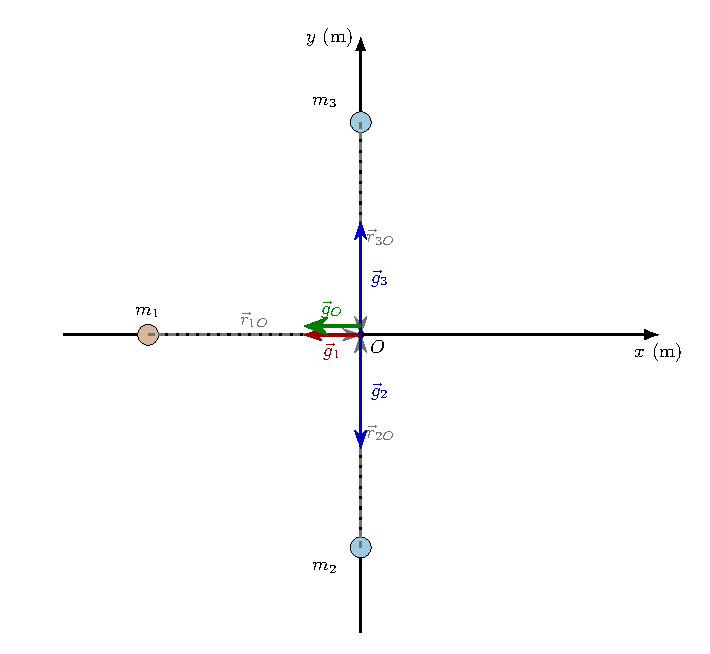
\includegraphics[width=0.8\linewidth]{SelectivosRESUELTOS2025/esquemas/Julio2013/1b(a).pdf}
    }}
    \caption{Superposición de los campos gravitatorios en el origen O.}
\end{figure}

\begin{figure}[H]
    \centering
    \fbox{\parbox{0.7\textwidth}{\centering \textbf{b) Potencial gravitatorio en P} \vspace{0.5cm} 
    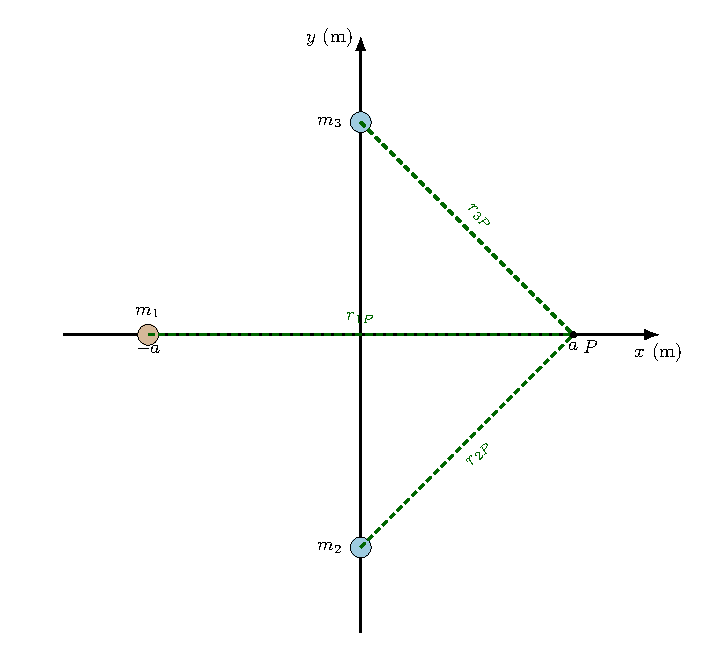
\includegraphics[width=0.8\linewidth]{SelectivosRESUELTOS2025/esquemas/Julio2013/1b(b).pdf}
    }}
    \caption{Distancias para el cálculo del potencial gravitatorio en el punto P.}
\end{figure}

\subsubsection*{3. Leyes y Fundamentos Físicos}
\paragraph{a) Campo Gravitatorio}
Se aplica el \textbf{Principio de Superposición}. El campo gravitatorio total en el origen O es la suma vectorial de los campos creados por cada masa: $\vec{g}_O = \vec{g}_1 + \vec{g}_2 + \vec{g}_3$. El campo creado por una masa puntual M es $\vec{g} = -G\frac{M}{r^2}\vec{u}_r$, donde $\vec{u}_r$ es el vector unitario que va desde la masa al punto.

\paragraph{b) Potencial Gravitatorio}
El potencial gravitatorio es una magnitud escalar. El potencial total en el punto P es la suma algebraica de los potenciales creados por cada masa: $V_P = V_1 + V_2 + V_3$. El potencial creado por una masa puntual es $V = -G\frac{M}{r}$.

\subsubsection*{4. Tratamiento Simbólico de las Ecuaciones}
\paragraph{a) Campo gravitatorio en O(0,0)}
\begin{itemize}
    \item \textbf{Campo de $m_1$ en O:} $\vec{g}_1 = -G\frac{m_1}{a^2}(-\vec{i}) = G\frac{m_1}{a^2}\vec{i}$.
    \item \textbf{Campo de $m_2$ en O:} $\vec{g}_2 = -G\frac{m_2}{a^2}(-\vec{j}) = G\frac{m_2}{a^2}\vec{j}$.
    \item \textbf{Campo de $m_3$ en O:} $\vec{g}_3 = -G\frac{m_3}{a^2}(\vec{j}) = -G\frac{m_3}{a^2}\vec{j}$.
\end{itemize}
Como $m_2=m_3$, los campos $\vec{g}_2$ y $\vec{g}_3$ son de igual módulo y sentido opuesto, por lo que se anulan.
$\vec{g}_O = \vec{g}_1 + \vec{g}_2 + \vec{g}_3 = \vec{g}_1$.

\paragraph{b) Potencial en P(a,0)}
Necesitamos las distancias de cada masa a P:
\begin{itemize}
    \item Distancia de $m_1$ a P: $r_{1P} = a - (-a) = 2a$.
    \item Distancia de $m_2$ a P: $r_{2P} = \sqrt{(a-0)^2 + (0-(-a))^2} = \sqrt{a^2+a^2} = a\sqrt{2}$.
    \item Distancia de $m_3$ a P: $r_{3P} = \sqrt{(a-0)^2 + (0-a)^2} = \sqrt{a^2+a^2} = a\sqrt{2}$.
\end{itemize}
$V_P = -G\frac{m_1}{r_{1P}} -G\frac{m_2}{r_{2P}} -G\frac{m_3}{r_{3P}}$.

\subsubsection*{5. Sustitución Numérica y Resultado}
\paragraph{a) Campo gravitatorio en O(0,0)}
\begin{gather}
    \vec{g}_O = G\frac{m_1}{a^2}\vec{i} = (6,67 \cdot 10^{-11})\frac{1 \cdot 10^{21}}{(10^5)^2}\vec{i} = (6,67 \cdot 10^{-11})\frac{10^{21}}{10^{10}}\vec{i} \nonumber \\
    \vec{g}_O = 6,67 \cdot 10^{-11} \cdot 10^{11} \vec{i} = 6,67\vec{i}\,\text{N/kg}
\end{gather}
\begin{cajaresultado}
El vector campo gravitatorio en el origen es $\boldsymbol{\vec{g}_O = 6,67\vec{i}\,\textbf{N/kg}}$.
\end{cajaresultado}

\paragraph{b) Potencial en P(a,0)}
\begin{gather}
    V_P = -G \left( \frac{m_1}{2a} + \frac{m_2}{a\sqrt{2}} + \frac{m_3}{a\sqrt{2}} \right) = -G \left( \frac{1 \cdot 10^{21}}{2 \cdot 10^5} + \frac{2 \cdot 10^{21}}{10^5\sqrt{2}} + \frac{2 \cdot 10^{21}}{10^5\sqrt{2}} \right) \nonumber \\
    V_P = -(6,67 \cdot 10^{-11}) \left( \frac{10^{16}}{2} + \frac{4 \cdot 10^{16}}{\sqrt{2}} \right) = -(6,67 \cdot 10^{-11}) \cdot 10^{16} \left( 0,5 + 2\sqrt{2} \right) \nonumber \\
    V_P \approx -(6,67 \cdot 10^{-11}) \cdot 10^{16} \cdot (3,328) \approx -2,22 \cdot 10^5\,\text{J/kg}
\end{gather}
\begin{cajaresultado}
El potencial gravitatorio en el punto P es $\boldsymbol{V_P \approx -2,22 \cdot 10^5\,\textbf{J/kg}}$.
\end{cajaresultado}

\subsubsection*{6. Conclusión}
\begin{cajaconclusion}
Debido a la simetría de las masas $m_2$ y $m_3$ respecto al eje X, sus contribuciones al campo gravitatorio en el origen se cancelan mutuamente, resultando un campo neto debido únicamente a la masa $m_1$. Para el cálculo del potencial en P, una magnitud escalar, se suman algebraicamente las contribuciones de las tres masas, resultando en un valor negativo, como corresponde al potencial gravitatorio.
\end{cajaconclusion}

\newpage

\subsection{Bloque II - Cuestión}
\label{subsec:B2_2013_jul_ext}

\begin{cajaenunciado}
Una onda longitudinal, de frecuencia 40 Hz, se propaga en un medio homogéneo. La distancia mínima entre dos puntos del medio con la misma fase es de 25 cm. Calcula la velocidad de propagación de la onda.
\end{cajaenunciado}
\hrule

\subsubsection*{1. Tratamiento de datos y lectura}
\begin{itemize}
    \item \textbf{Frecuencia de la onda ($f$):} $f = 40\,\text{Hz}$.
    \item \textbf{Distancia mínima entre puntos en fase:} Esta distancia es, por definición, la longitud de onda ($\lambda$).
    $\lambda = 25\,\text{cm} = 0,25\,\text{m}$.
    \item \textbf{Incógnita:} Velocidad de propagación de la onda ($v$).
\end{itemize}

\subsubsection*{2. Representación Gráfica}
\begin{figure}[H]
    \centering
    \fbox{\parbox{0.8\textwidth}{\centering 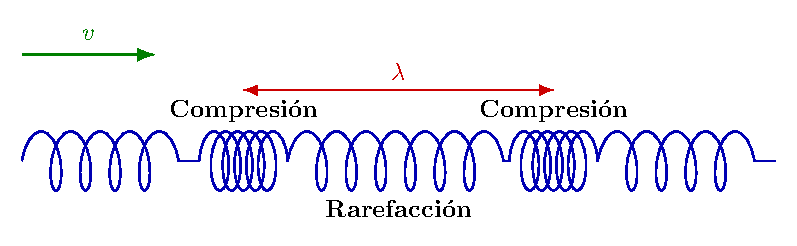
\includegraphics[width=0.9\linewidth]{SelectivosRESUELTOS2025/esquemas/Julio2013/2b.pdf}
    }}
    \caption{Representación de la longitud de onda en una onda longitudinal.}
\end{figure}

\subsubsection*{3. Leyes y Fundamentos Físicos}
La relación entre la velocidad de propagación de una onda ($v$), su longitud de onda ($\lambda$) y su frecuencia ($f$) viene dada por la ecuación fundamental de las ondas:
$$ v = \lambda \cdot f $$
Esta relación es válida para todo tipo de ondas armónicas, tanto longitudinales como transversales.

\subsubsection*{4. Tratamiento Simbólico de las Ecuaciones}
La ecuación a utilizar es directamente la ecuación fundamental de las ondas. No requiere manipulación algebraica.
\begin{gather}
    v = \lambda \cdot f
\end{gather}

\subsubsection*{5. Sustitución Numérica y Resultado}
Sustituimos los datos del problema, asegurándonos de que están en unidades del Sistema Internacional.
\begin{gather}
    v = (0,25\,\text{m}) \cdot (40\,\text{Hz}) = 10\,\text{m/s}
\end{gather}
\begin{cajaresultado}
La velocidad de propagación de la onda es $\boldsymbol{v = 10\,\textbf{m/s}}$.
\end{cajaresultado}

\subsubsection*{6. Conclusión}
\begin{cajaconclusion}
La distancia mínima entre dos puntos en fase define la longitud de onda. Conociendo la longitud de onda (0,25 m) y la frecuencia (40 Hz), la velocidad de propagación se calcula directamente a partir de la ecuación fundamental de las ondas, resultando en 10 m/s.
\end{cajaconclusion}

\newpage

\subsection{Bloque III - Problema}
\label{subsec:B3_2013_jul_ext}

\begin{cajaenunciado}
Un rayo de luz monocromática atraviesa el vidrio de una ventana que separa dos ambientes en los que el medio es el aire. Si el espesor del vidrio es de 6 mm y el rayo incide con un ángulo de 30° respecto a la normal:
\begin{enumerate}
    \item[a)] Dibuja el esquema de la trayectoria del rayo y calcula la longitud de ésta en el interior del vidrio. (1,2 puntos)
    \item[b)] Calcula el ángulo que forman las direcciones de los rayos incidente y emergente en el aire. (0,8 puntos)
\end{enumerate}
\textbf{Dato:} índice de refracción del vidrio, $n=1,5$.
\end{cajaenunciado}
\hrule

\subsubsection*{1. Tratamiento de datos y lectura}
\begin{itemize}
    \item \textbf{Medio inicial y final:} Aire, cuyo índice de refracción es $n_1 = n_3 \approx 1$.
    \item \textbf{Medio intermedio:} Vidrio, con índice de refracción $n_2 = 1,5$.
    \item \textbf{Espesor del vidrio ($e$):} $e = 6\,\text{mm} = 6 \cdot 10^{-3}\,\text{m}$.
    \item \textbf{Ángulo de incidencia inicial ($\theta_1$):} $\theta_1 = 30^\circ$.
    \item \textbf{Incógnitas:}
        \begin{itemize}
            \item[a)] Esquema y longitud del camino en el vidrio ($L$).
            \item[b)] Ángulo entre el rayo incidente y el emergente.
        \end{itemize}
\end{itemize}

\subsubsection*{2. Representación Gráfica}
\begin{figure}[H]
    \centering
    \fbox{\parbox{0.8\textwidth}{\centering 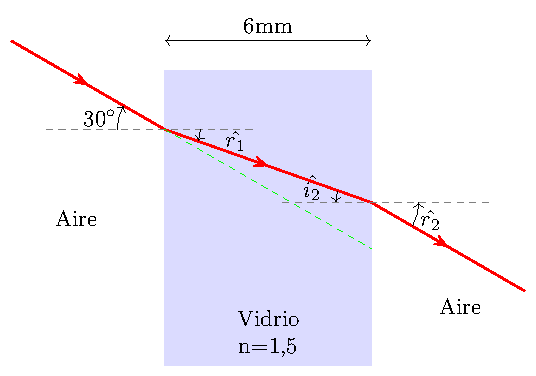
\includegraphics[width=0.9\linewidth]{SelectivosRESUELTOS2025/esquemas/Julio2013/3b.pdf}
    }}
    \caption{a) Esquema de la trayectoria del rayo de luz a través del vidrio.}
\end{figure}

\subsubsection*{3. Leyes y Fundamentos Físicos}
\paragraph{a) Longitud de la trayectoria}
El problema se resuelve aplicando la \textbf{Ley de Snell de la refracción} en la primera interfaz (aire-vidrio) para encontrar el ángulo de refracción $\theta_2$. Una vez conocido $\theta_2$, la longitud del camino del rayo dentro del vidrio ($L$) se puede obtener mediante relaciones trigonométricas en el triángulo rectángulo que forma el rayo con la normal y el espesor del vidrio.

\paragraph{b) Ángulo entre rayos}
Se aplica de nuevo la Ley de Snell en la segunda interfaz (vidrio-aire) para encontrar el ángulo de emergencia $\theta_3$. El ángulo que forman los rayos incidente y emergente es la diferencia entre sus direcciones. Si resultan ser paralelos, este ángulo será de 0°.

\subsubsection*{4. Tratamiento Simbólico de las Ecuaciones}
\paragraph{a) Ángulo de refracción y longitud}
Aplicamos Snell en la primera cara:
\begin{gather}
    n_1 \sin(\theta_1) = n_2 \sin(\theta_2) \implies \theta_2 = \arcsin\left(\frac{n_1 \sin(\theta_1)}{n_2}\right)
\end{gather}
Del triángulo rectángulo dentro del vidrio, se tiene:
\begin{gather}
    \cos(\theta_2) = \frac{\text{cateto contiguo}}{\text{hipotenusa}} = \frac{e}{L} \implies L = \frac{e}{\cos(\theta_2)}
\end{gather}

\paragraph{b) Ángulo de emergencia}
Aplicamos Snell en la segunda cara. El ángulo de incidencia es $\theta_2$:
\begin{gather}
    n_2 \sin(\theta_2) = n_3 \sin(\theta_3)
\end{gather}
Como $n_1 = n_3$ (aire en ambos lados), y de la primera refracción sabemos que $n_1 \sin(\theta_1) = n_2 \sin(\theta_2)$, podemos concluir que $n_1 \sin(\theta_1) = n_1 \sin(\theta_3)$, lo que implica $\theta_1 = \theta_3$.

\subsubsection*{5. Sustitución Numérica y Resultado}
\paragraph{a) Cálculo de la longitud}
Primero calculamos $\theta_2$:
\begin{gather}
    1 \cdot \sin(30^\circ) = 1,5 \cdot \sin(\theta_2) \implies \sin(\theta_2) = \frac{0,5}{1,5} = \frac{1}{3} \nonumber \\
    \theta_2 = \arcsin(1/3) \approx 19,47^\circ
\end{gather}
Ahora calculamos la longitud $L$:
\begin{gather}
    L = \frac{6\,\text{mm}}{\cos(19,47^\circ)} \approx \frac{6\,\text{mm}}{0,9428} \approx 6,36\,\text{mm}
\end{gather}
\begin{cajaresultado}
La longitud de la trayectoria del rayo en el interior del vidrio es $\boldsymbol{L \approx 6,36\,\textbf{mm}}$.
\end{cajaresultado}

\paragraph{b) Cálculo del ángulo}
Como hemos deducido simbólicamente, al ser el medio inicial y final el mismo (aire), el rayo emergente sale con el mismo ángulo que el rayo incidente: $\theta_3 = \theta_1 = 30^\circ$. Esto significa que los rayos incidente y emergente son paralelos entre sí.
\begin{cajaresultado}
El rayo emergente es paralelo al incidente, por lo que el ángulo que forman sus direcciones es de $\boldsymbol{0^\circ}$.
\end{cajaresultado}

\subsubsection*{6. Conclusión}
\begin{cajaconclusion}
Al atravesar la lámina de vidrio, el rayo de luz sufre dos refracciones. Se ha calculado que la trayectoria dentro del vidrio tiene una longitud de 6,36 mm. Al emerger de nuevo al aire, el rayo recupera su dirección original, resultando en un rayo emergente paralelo al incidente. Aunque no se pregunta, el rayo emergente ha sufrido un desplazamiento lateral respecto a la prolongación del rayo incidente.
\end{cajaconclusion}

\newpage

\subsection{Bloque IV - Cuestión}
\label{subsec:B4_2013_jul_ext}

\begin{cajaenunciado}
Una espira conductora, con forma circular, está situada en el seno de un campo magnético perpendicular al plano del papel, como muestra la figura. El módulo del campo magnético aumenta con el tiempo. Indica el sentido de la corriente inducida en la espira y justifica la respuesta basándote en las leyes que explican este fenómeno.
\end{cajaenunciado}
\hrule

\subsubsection*{1. Tratamiento de datos y lectura}
\begin{itemize}
    \item \textbf{Circuito:} Espira circular conductora.
    \item \textbf{Campo magnético externo ($\vec{B}_{ext}$):} Uniforme, perpendicular al plano de la espira y dirigido hacia dentro del papel (indicado por las cruces).
    \item \textbf{Variación del campo:} Su módulo, $B_{ext}$, aumenta con el tiempo.
    \item \textbf{Incógnita:} Sentido de la corriente inducida ($I_{ind}$).
\end{itemize}

\subsubsection*{2. Representación Gráfica}
\begin{figure}[H]
    \centering
    \fbox{\parbox{0.6\textwidth}{\centering  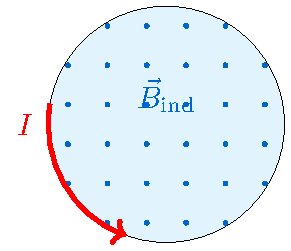
\includegraphics[width=0.6\linewidth]{SelectivosRESUELTOS2025/esquemas/Julio2013/4b.pdf}
    }}
    \caption{Determinación del sentido de la corriente inducida.}
\end{figure}

\subsubsection*{3. Leyes y Fundamentos Físicos}
El fenómeno se explica por la \textbf{Ley de Faraday-Lenz de la inducción electromagnética}.
\begin{itemize}
    \item \textbf{Ley de Faraday:} Establece que una variación en el flujo magnético ($\Phi_B$) a través de una espira induce una fuerza electromotriz (fem, $\varepsilon$) en ella: $\varepsilon = -d\Phi_B/dt$.
    \item \textbf{Ley de Lenz:} Es la responsable del signo negativo y proporciona el sentido de la corriente inducida. Afirma que la corriente inducida circulará en un sentido tal que el campo magnético que ella misma crea se opone a la variación del flujo magnético que la originó. Es, en esencia, una manifestación del principio de conservación de la energía.
\end{itemize}

\subsubsection*{4. Tratamiento Simbólico de las Ecuaciones}
El flujo magnético a través de la espira es $\Phi_B = \vec{B}_{ext} \cdot \vec{S} = B_{ext} S \cos(0^\circ) = B_{ext} S$.
Como el área $S$ es constante pero $B_{ext}$ aumenta con el tiempo, la derivada del flujo respecto al tiempo es positiva:
\begin{gather}
    \frac{d\Phi_B}{dt} = S \frac{dB_{ext}}{dt} > 0
\end{gather}
Según la ley de Faraday-Lenz, se induce una fem y por tanto una corriente. El sentido de esta corriente debe ser tal que cree un campo magnético inducido, $\vec{B}_{ind}$, que genere un flujo que se oponga al aumento.

\subsubsection*{5. Sustitución Numérica y Resultado}
El razonamiento es cualitativo:
\begin{enumerate}
    \item \textbf{Análisis de la variación del flujo:} El campo magnético externo apunta hacia \textbf{dentro} del papel y su módulo está \textbf{aumentando}. Por lo tanto, el flujo magnético hacia dentro del papel está aumentando.
    \item \textbf{Aplicación de la Ley de Lenz:} Para oponerse a este \textit{aumento de flujo hacia dentro}, la espira debe generar un campo magnético inducido, $\vec{B}_{ind}$, que apunte en sentido contrario, es decir, \textbf{hacia fuera} del papel.
    \item \textbf{Determinación del sentido de la corriente (Regla de la mano derecha):} Para que una corriente circular cree un campo magnético hacia fuera del papel en su interior, debe circular en sentido \textbf{antihorario}.
\end{enumerate}
\begin{cajaresultado}
El sentido de la corriente inducida en la espira es \textbf{antihorario}.
\end{cajaresultado}

\subsubsection*{6. Conclusión}
\begin{cajaconclusion}
La Ley de Lenz, que rige el sentido de la corriente inducida, puede verse como una "inercia electromagnética". El sistema se opone al cambio. Dado que el flujo magnético hacia el interior de la espira está aumentando, se induce una corriente antihoraria para generar un campo magnético propio hacia el exterior que contrarreste dicho aumento.
\end{cajaconclusion}

\newpage

\subsection{Bloque V - Cuestión}
\label{subsec:B5_2013_jul_ext}

\begin{cajaenunciado}
Una nave se aleja de la Tierra con una velocidad de $2 \cdot 10^8\,\text{m/s}$. A su vez, desde la Tierra se emite un haz de luz láser en dirección a la nave. ¿Cuál es la velocidad del haz láser para el observador de la nave? Justifica la respuesta.
\end{cajaenunciado}
\hrule

\subsubsection*{1. Tratamiento de datos y lectura}
\begin{itemize}
    \item \textbf{Observador 1:} Un observador en la Tierra.
    \item \textbf{Observador 2:} Un observador en una nave.
    \item \textbf{Velocidad relativa entre observadores:} $v = 2 \cdot 10^8\,\text{m/s}$.
    \item \textbf{Fenómeno observado:} Un haz de luz láser.
    \item \textbf{Incógnita:} Velocidad del haz láser medida por el observador en la nave.
\end{itemize}

\subsubsection*{2. Representación Gráfica}
\begin{figure}[H]
    \centering
    \fbox{\parbox{0.8\textwidth}{\centering 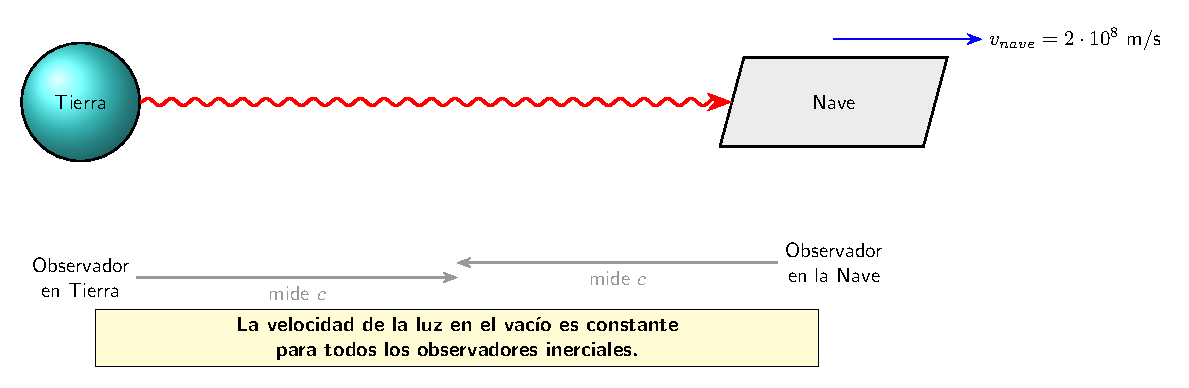
\includegraphics[width=0.9\linewidth]{SelectivosRESUELTOS2025/esquemas/Julio2013/5b.pdf}
    }}
    \caption{La velocidad de la luz es independiente del estado de movimiento del observador.}
\end{figure}

\subsubsection*{3. Leyes y Fundamentos Físicos}
La respuesta a esta pregunta se basa directamente en el \textbf{Segundo Postulado de la Teoría de la Relatividad Especial} de Albert Einstein.
\begin{itemize}
    \item \textbf{Postulado de la constancia de la velocidad de la luz:} La velocidad de la luz en el vacío tiene el mismo valor, $c$ (aproximadamente $3 \cdot 10^8\,\text{m/s}$), en todos los sistemas de referencia inerciales, independientemente del movimiento de la fuente de luz o del observador.
\end{itemize}
Este postulado es uno de los pilares de la física moderna y tiene consecuencias profundas, como la dilatación del tiempo y la contracción de la longitud. Contradice nuestra intuición basada en la mecánica clásica de Galileo, donde las velocidades se suman o restan.

\subsubsection*{4. Tratamiento Simbólico de las Ecuaciones}
No se requiere un tratamiento matemático. La respuesta es la aplicación directa del postulado.
La ley de adición de velocidades relativista es:
$$ u' = \frac{u-v}{1-uv/c^2} $$
Donde $u$ es la velocidad del objeto (el láser) medida desde la Tierra ($u=c$), $v$ es la velocidad de la nave, y $u'$ es la velocidad del láser medida desde la nave.
$$ u' = \frac{c-v}{1-cv/c^2} = \frac{c-v}{1-v/c} = \frac{c(1-v/c)}{(1-v/c)} = c $$
El formalismo matemático confirma el postulado.

\subsubsection*{5. Sustitución Numérica y Resultado}
Independientemente del valor de la velocidad de la nave ($v=2 \cdot 10^8\,\text{m/s}$), la velocidad de la luz medida por cualquier observador inercial es siempre la misma.
\begin{cajaresultado}
La velocidad del haz láser para el observador de la nave es $\boldsymbol{c = 3 \cdot 10^8\,\textbf{m/s}}$.
\end{cajaresultado}

\subsubsection*{6. Conclusión}
\begin{cajaconclusion}
A diferencia de los objetos materiales, cuya velocidad medida depende del sistema de referencia del observador, la velocidad de la luz en el vacío es una constante universal. Tanto un observador en reposo en la Tierra como un observador en la nave que se aleja a gran velocidad medirán exactamente el mismo valor, $c$, para la velocidad del haz de láser, tal y como postula la Relatividad Especial.
\end{cajaconclusion}

\newpage

\subsection{Bloque VI - Cuestión}
\label{subsec:B6_2013_jul_ext}

\begin{cajaenunciado}
Enuncia la hipótesis de De Broglie. Menciona un experimento que confirme dicha hipótesis, justificando la respuesta.
\end{cajaenunciado}
\hrule

\subsubsection*{1. Tratamiento de datos y lectura}
Es una cuestión teórica que requiere dos partes:
\begin{itemize}
    \item \textbf{Enunciado:} Formular la hipótesis de la dualidad onda-corpúsculo de De Broglie.
    \item \textbf{Confirmación experimental:} Citar un experimento histórico y explicar por qué confirma la hipótesis.
\end{itemize}

\subsubsection*{2. Representación Gráfica}
\begin{figure}[H]
    \centering
    \fbox{\parbox{0.8\textwidth}{\centering 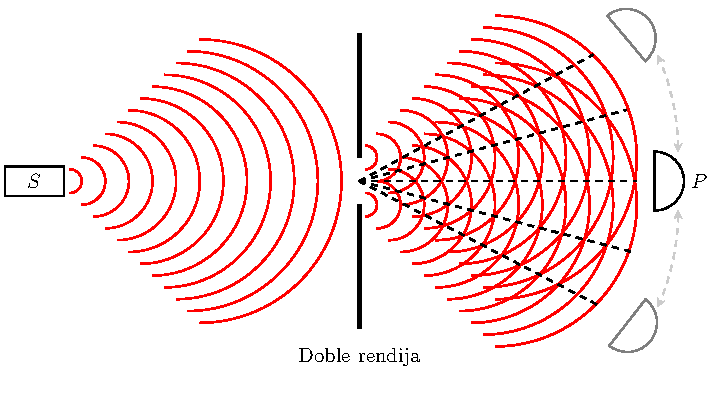
\includegraphics[width=0.9\linewidth]{SelectivosRESUELTOS2025/esquemas/Julio2013/6b.pdf}
    }}
    \caption{Esquema conceptual del experimento que confirmó la naturaleza ondulatoria de la materia.}
\end{figure}

\subsubsection*{3. Leyes y Fundamentos Físicos}
\paragraph{Enunciado de la Hipótesis de De Broglie}
En 1924, Louis de Broglie, extendiendo la dualidad onda-corpúsculo de la luz a la materia, postuló que \textbf{toda partícula en movimiento lleva asociada una onda}. La longitud de esta "onda de materia" es inversamente proporcional al momento lineal ($p$) de la partícula. Esta hipótesis unifica los conceptos de partícula y onda para toda la materia y energía.
La expresión matemática es:
$$ \lambda = \frac{h}{p} = \frac{h}{mv} $$
donde $\lambda$ es la longitud de onda de De Broglie, $h$ es la constante de Planck, $m$ es la masa de la partícula y $v$ su velocidad.

\paragraph{Experimento de Confirmación: La Difracción de Electrones}
El experimento más famoso que confirmó la hipótesis de De Broglie fue el realizado por \textbf{Clinton Davisson y Lester Germer} en 1927.
\begin{itemize}
    \item \textbf{Procedimiento:} Dispararon un haz de electrones de energía conocida contra la superficie de un cristal de níquel.
    \item \textbf{Observación:} En lugar de rebotar de forma dispersa como se esperaría de pequeñas partículas, los electrones emergían en direcciones muy específicas, formando un patrón de máximos y mínimos de intensidad, similar al patrón de difracción que se obtiene cuando los rayos X (que son ondas) atraviesan un cristal.
    \item \textbf{Justificación:} La difracción y la interferencia son fenómenos exclusivamente ondulatorios. El hecho de que un haz de electrones produjera un patrón de difracción era una prueba irrefutable de su comportamiento ondulatorio. Además, al tratar los átomos del cristal como una red de difracción, pudieron calcular la longitud de onda de los electrones a partir del patrón observado. El valor experimental coincidía perfectamente con la longitud de onda teórica predicha por la fórmula de De Broglie ($\lambda=h/p$).
\end{itemize}

\subsubsection*{4. Tratamiento Simbólico de las Ecuaciones}
La ecuación fundamental es la de De Broglie:
\begin{gather}
    \lambda = \frac{h}{p}
\end{gather}

\subsubsection*{5. Sustitución Numérica y Resultado}
No aplica, es una cuestión teórica.
\begin{cajaresultado}
\textbf{Hipótesis:} Toda partícula en movimiento (masa $m$, velocidad $v$) tiene una longitud de onda asociada $\lambda = h/p$.
\textbf{Confirmación:} El \textbf{experimento de Davisson y Germer}, que demostró que los electrones son difractados por un cristal, un fenómeno característico de las ondas, y cuya longitud de onda medida coincidía con la predicha por De Broglie.
\end{cajaresultado}

\subsubsection*{6. Conclusión}
\begin{cajaconclusion}
La audaz hipótesis de De Broglie, que atribuye propiedades ondulatorias a partículas como los electrones, fue un pilar fundamental en el desarrollo de la mecánica cuántica. El experimento de Davisson y Germer proporcionó la evidencia experimental concluyente de esta dualidad onda-corpúsculo para la materia, cambiando para siempre nuestra comprensión de la naturaleza fundamental del universo.
\end{cajaconclusion}

\newpage
